%+------------------------------------------------------------------------+
%| Diagram: HCMM as a Lift
%| Author: Antonio miti
%+------------------------------------------------------------------------+


\documentclass[beamer]{standalone}
\usepackage{tikz-cd}
\usepackage{mathtools}
\usepackage{amsfonts}
\usepackage{tikz}
\usetikzlibrary{calc}

\begin{document}
			\only<1>{
			\resizebox{\textwidth}{!}{
				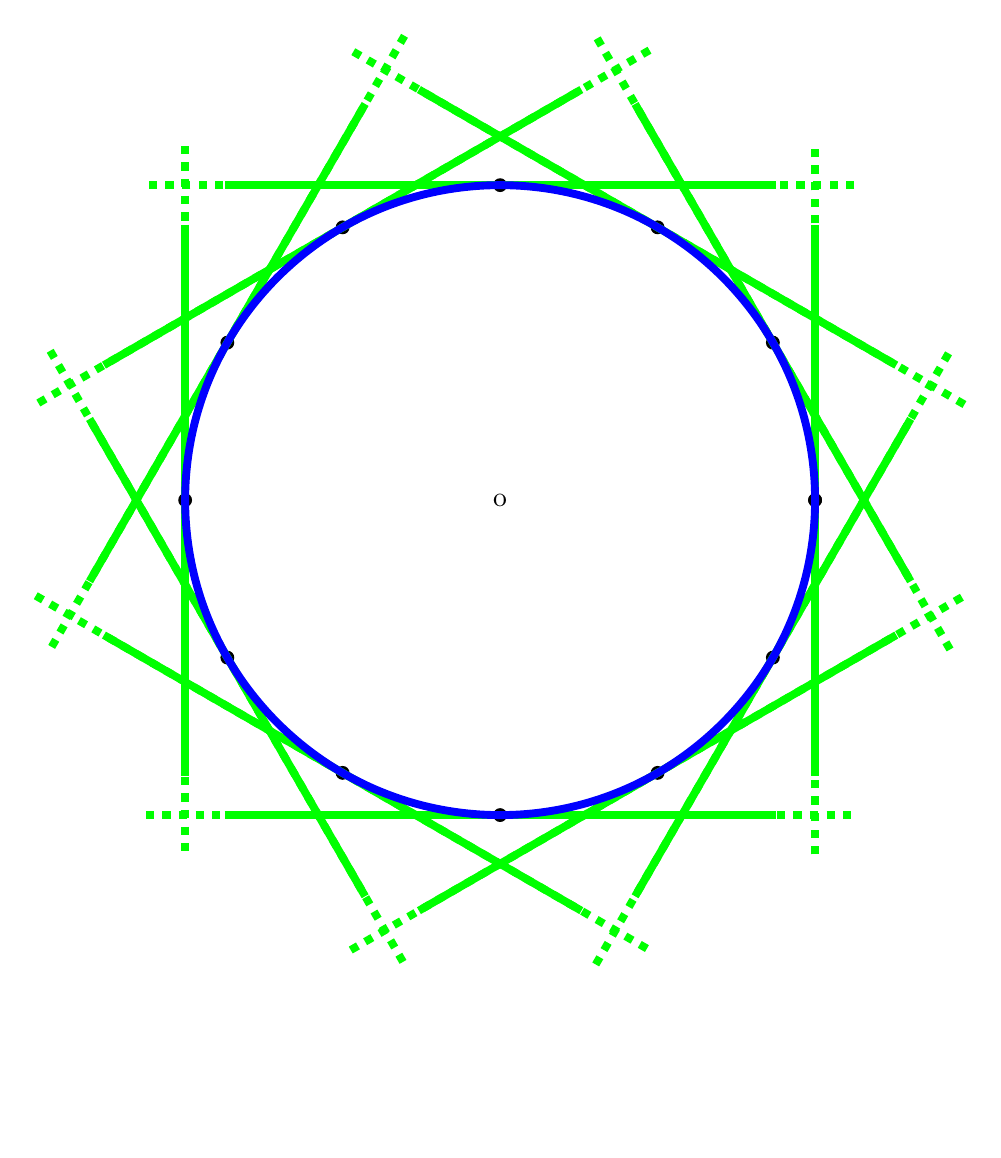
\begin{tikzpicture}
					\node[draw=none] (o) at (0, 0) {o};
				    %frame
				    \draw[draw=none] (-6,-8) rectangle (6,6);						
					\foreach \x in {0,30,...,360}{
						\draw[draw=none](0,0)--(\x:4)node[circle, fill, minimum size=5pt,
					              inner sep=0pt, outer sep=0pt](p){};
					\draw[green,line width=1mm] ($ (p)!3.5cm!90:(o) $) -- ($ (p)!3.5cm!270:(o) $);
					\draw[green,dashed,line width=1mm] ($ (p)!4.5cm!90:(o) $) -- ($ (p)!4.5cm!270:(o) $);
					}
						\draw[blue,line width=1mm] (0,0) circle (4);
				\end{tikzpicture}
			}}
			%
			\only<2->{
			\resizebox{.7\textwidth}{!}{
				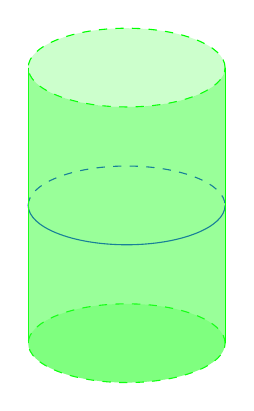
\begin{tikzpicture}
					\draw[green,dashed,fill=green!20] (0,0) ellipse (1.25 and 0.5);
					\draw [blue](-1.25,-1.75) arc (180:360:1.25 and 0.5);
					%\draw [blue,dashed] (-1.25,-3.5) arc (180:360:1.25 and -0.5);
					\draw[green,dashed,fill=green!20] (0,-3.5) ellipse (1.25 and 0.5);
					\draw [blue,dashed] (-1.25,-1.75) arc (180:360:1.25 and -0.5);
					\draw [green](-1.25,0) -- (-1.25,-3.5);
					\draw [green](1.25,-3.5) -- (1.25,0);  
					\fill [green!80,opacity=0.5] (-1.25,0) -- (-1.25,-3.5) arc (180:360:1.25 and 0.5) -- (1.25,0) arc (0:180:1.25 and -0.5);
				\end{tikzpicture}		
%				\begin{tikzpicture}
%				  \node[cylinder,draw=black,thick,aspect=0.7,minimum height=4cm,minimum width=2.5cm,shape border rotate=90,cylinder uses custom fill, cylinder body fill=green!30,cylinder end fill=green!10] (A) {\phantom{A}};
%				  \draw[dashed]
%				    let \p1 = ($ (A.after bottom) - (A.before bottom) $),
%				        \n1 = {0.5*veclen(\x1,\y1)-\pgflinewidth},
%				        \p2 = ($ (A.bottom) - (A.after bottom)!.5!(A.before bottom) $),
%				        \n2 = {veclen(\x2,\y2)-\pgflinewidth}
%				  in
%				    ([xshift=-\pgflinewidth] A.before bottom) arc [start angle=0, end angle=180,
%				    x radius=\n1, y radius=\n2];
%				\end{tikzpicture}	
}
			}
\end{document}

